\documentclass{article}
\usepackage[spanish]{babel}
\usepackage[utf8]{inputenc}
\usepackage{graphicx}
\usepackage{listings}
\usepackage{xcolor}
\usepackage{hyperref}
\usepackage{caption}
\usepackage[skip=5pt]{parskip}
\usepackage{bytefield}

\lstset{
    basicstyle=\ttfamily\small,
    frame=lines,
    framesep=2mm,
    backgroundcolor=\color{gray!5},
    rulecolor=\color{gray},
    breaklines=true
}



\begin{document}
\begin{titlepage}
    \centering
    {\large \textbf{Instituto Politecnico Superior "General San Martin"}}\\[1.5cm] 
    {\huge \textbf{Protocolo IPv6}}\\[1.5cm]
    
    \textbf{Materia:} Administración de Redes Locales\\[0.5cm]
    \textbf{Profesor:} Alejandro Rodríguez Costello\\[1.5cm]
    
    \textbf{Integrantes del grupo:}\\
    Gerónimo Chávarri\\
    Ignacio Tasada\\
    Manuel Ferrer Petit\\[1.5cm]
    
    \textbf{Link del Repositorio Github:}\\
    \href{https://github.com/GeroTxbarri/Trabajo-Practico-Redes-El-protocolo-IPv6.git}{https://github.com/GeroTxbarri/Trabajo-Practico-Redes-El-protocolo-IPv6.git}\\[2cm]
    
    
\end{titlepage}

\maketitle

\section{IPv6 SLAAC and EUI-64 Basics:Configuración del router en IPv6}
Creamos un nuevo escenario usando un router 1941, un switch 2960 y una PC como se observa en la figura:

\begin{figure}[h]
    \centering
    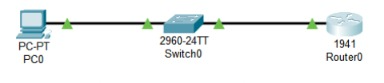
\includegraphics[width=0.8\textwidth]{img 1 coba.png}
    \caption{Escenario de laboratorio}
\end{figure}

El objetivo es ver como PC0 se autoconfigura usando SLAAC en IPv6. Para ello activamos el ruteo IPv6 en Router0 en el modo global config con:

\begin{lstlisting}
Router(config)#ipv6 unicast-routing
\end{lstlisting}

Ahora habilitamos la interface g0/0 con IPv6 y dos direcciones:
\begin{itemize}
    \item Una local llamada LLA (Local Link Address) \texttt{FE80::1}
    \item Otra global \texttt{2001:DB8:ACAD:1::1/64} o ruteable llamada GUA (Global Unicast Address)
\end{itemize}
\begin{figure}[h]
    \centering
    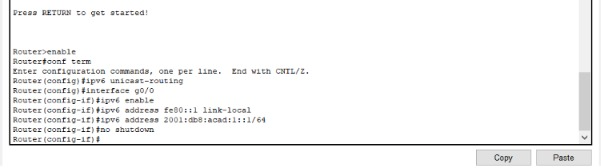
\includegraphics[width=0.8\textwidth]{imgcob2.png}
    \caption{Escenario de laboratorio}
\end{figure}

Ahora pasamos a modo Simulation y abrimos en la pestaña Desktop de la PC0 la aplicación IP Configuration y tomamos nota de la LLA en la seccion IPv6 Configuration como se observa y la comparamos con la dirección MAC que se puede obtener en Config > FastEthernet0. Explique su relación usando el algoritmo de EUI-64.

\begin{figure}[h]
    \centering
    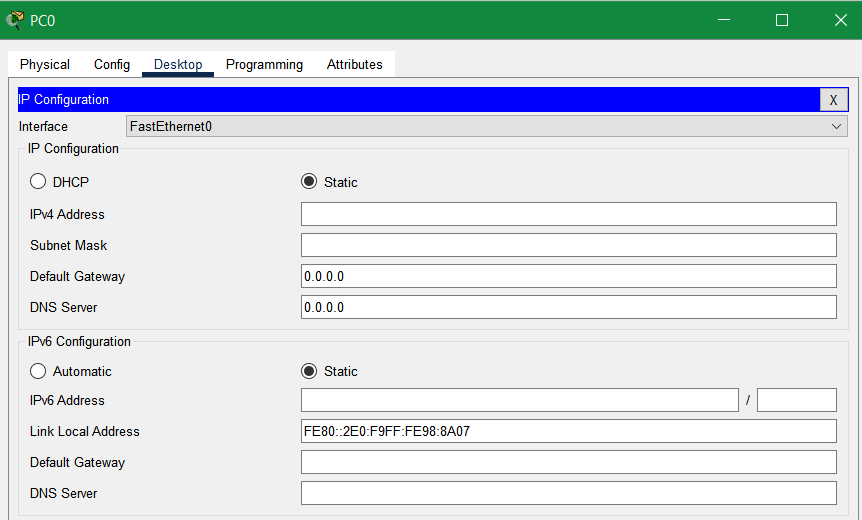
\includegraphics[width=0.8\textwidth]{1.png}
\end{figure}
\begin{figure}[h]
    \centering
    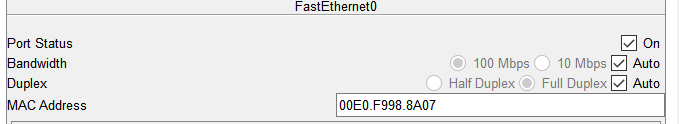
\includegraphics[width=0.8\textwidth]{2.png}
\end{figure}



\begin{itemize}
    \item Dirección LLA: \texttt{FE80::2E0:F9FF:FE98:8A07}
    \item Dirección Mac: \texttt{00E0.F998.8A07}
\end{itemize}

Podemos ver el LLA de la pc se configuró automáticamente utilizando el método EUI-64, es decir, se convirtió una dirección mac de 48 bits en una ipv6 de 64 bit

\subsection*{Explicación}
Mac: \texttt{00E0.F998.8A07}

Se la divide en dos: \texttt{00E0.F9} \hspace{5mm} \texttt{98.8A07}

Se inserta FFFE en el medio: \texttt{00E0.F9FF.FE98.8A07}

Inversion 7mo bit: \texttt{00E0} $\rightarrow$ \texttt{00000010} $\rightarrow$ \texttt{02E0}

Prefijo: \texttt{FE80::/64}

dirección LLA: \texttt{FE80::2E0:F9FF:FE98:8A07}

Ahora pasamos de Static a Automatic y sin cerrar esta ventana nos concentramos en el Simulation Panel1. Como se observa en la figura 3, la PC0 emite un mensaje NDP. Abra el PDU para obtener detalles y explique cuales son los campos relevantes del mensaje tipo RS (Router Solicitation).


\begin{bytefield}{32}
    \bitheader{0-31} \\ % Encabezado de bits
    \bitbox{4}{VER: 6} & \bitbox{8}{TRFC} & \bitbox{20}{FLOW LABEL} \\
    \bitbox{16}{PL: 12} & \bitbox{8}{NEXT: 0x3a} & \bitbox{8}{HOP LIMIT: 255} \\
    \bitbox{32}{SRC IP: FE80::2E0:F9FF:FE98:8A07} \\
    \wordbox{1}{ } \\
    \wordbox{1}{ } \\
    \bitbox{32}{DST IP: FF02::2} \\
\end{bytefield}
\begin{figure}[h]
    \centering
    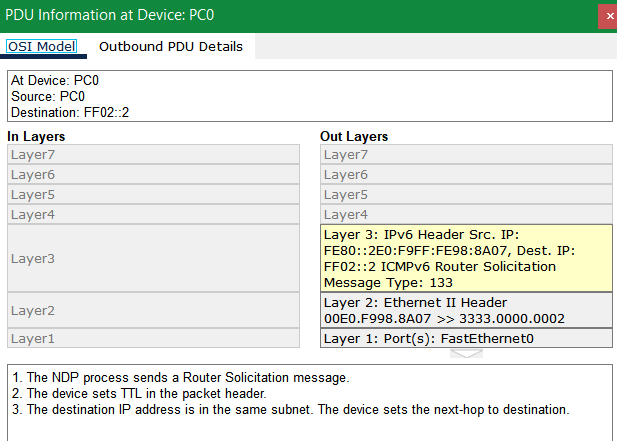
\includegraphics[width=0.8\textwidth]{5.png}
\end{figure}

\begin{figure}[h]
    \centering
    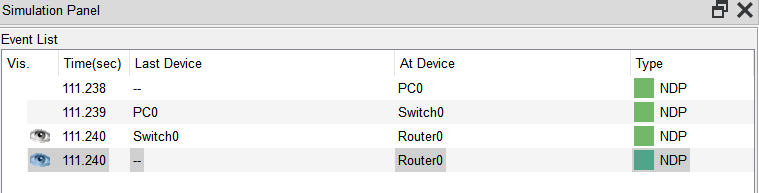
\includegraphics[width=0.8\textwidth]{6.png}
\end{figure}


\begin{itemize}
    \item Message type: 133 (Indica que es un Router Solicitation, RS)
    \item Dirección de destino: \texttt{FF02::2} (Multicast a todos los routers en la red local)
    \item Dirección de Origen: \texttt{FE80::2E0:F9FF:FE98:8A07} (Dirección LLA de la PC0)
    \item Hop limit: 255
\end{itemize}

Luego avance con el botón forward hasta que el mensaje de respuesta arribe a la PC0 y analice el PDU de respuesta tipo RA (Router Advertising). Compruebe que la PC ahora tiene una dirección GUA y cual es la misma y explique cómo la obtuvo a través de la información analizada.
\begin{figure}[h]
    \centering
    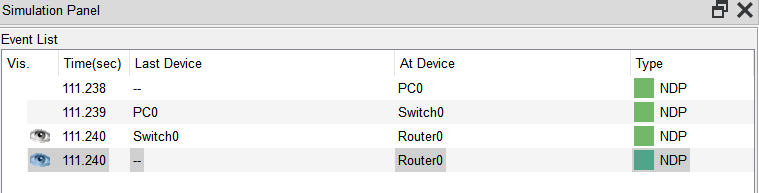
\includegraphics[width=0.8\textwidth]{6.png}
\end{figure}
\begin{figure}[h]
    \centering
    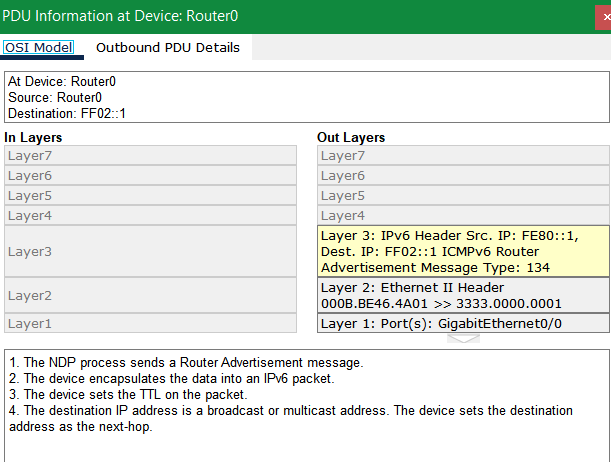
\includegraphics[width=0.8\textwidth]{7.png}
\end{figure}


\begin{bytefield}{32}
    \bitheader{0-31} \\ % Encabezado de bits
    \bitbox{4}{VER: 6} & \bitbox{8}{TRFC} & \bitbox{20}{FLOW LABEL} \\
    \bitbox{16}{PL: 60} & \bitbox{8}{NEXT: 0x3a} & \bitbox{8}{HOP LIMIT: 255} \\
    \bitbox{32}{SRC IP: FE80::1} \\
\end{bytefield}

\begin{itemize}
    \item Message Type: 134 (Indica que es un Router Advertisement, RA)
    \item Dirección de origen: \texttt{FE80::1} (LLA del router en g0/0)
    \item Direccion de Destino: \texttt{FF02::1} (Multicast a todos los nodos de la red)
    \item Hop limit: 255
    \item Dirección GUA de pc0: \texttt{2001:DB8:ACAD:1:2E0:F9FF:FE98:8A07}
\end{itemize}

\subsection*{Explicación:}
La PC recibe el prefijo de red \texttt{2001:DB8:ACAD:1::/64} desde el mensaje RA.

Aplica SLAAC para autogenerar su dirección:

Usa el prefijo del router (\texttt{2001:DB8:ACAD:1::/64}).

Usa el método EUI-64 para derivar su identificador de host (como hicimos antes con la LLA).

Dirección resultante: \texttt{2001:DB8:ACAD:1:2E0:F9FF:FE98:8A07}

\section{Neighbor Discovery}
Debido a que IPv6 no utiliza ARP es necesario un mecanismo para obtener las direcciones MAC. Para ello utilizaremos el escenario de la figura 4 con las direcciones IPv6 configuradas como indica la tabla siguiente:
\begin{figure}[h]
    \centering
    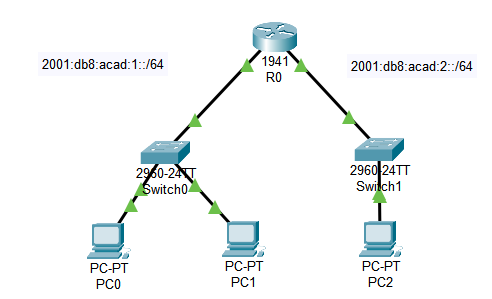
\includegraphics[width=0.8\textwidth]{9.png}
\end{figure}


\begin{table}[h]
\centering
\caption{Configuración de direcciones IPv6}
\begin{tabular}{ll}
\toprule
Dispositivo & Dirección IPv6 \\
\midrule
PC0 & \dir{2001:DB8:ACAD:1::A} \\
PC1 & \dir{2001:DB8:ACAD:1::B} \\
Router0 & \dir{2001:DB8:ACAD:1::1} \\
\bottomrule
\end{tabular}
\end{table}

\subsection{Local delivery}
Aunque el mecanismo a estudiar es similar para la mayoría de los casos, es importante diferenciar cómo opera NDP a nivel red local respecto del envío a otras redes remotas como se hizo en ARP para IPv4. Para ello nos aseguramos que R0 no contiene información de sus vecinos con:

\begin{lstlisting}
R0#show ipv6 neighbors
\end{lstlisting}

Si hubiera alguna salida utilizaremos:

\begin{lstlisting}
R0#clear ipv6 neighbors
\end{lstlisting}

Ahora en modo simulación vamos a filtrar los mensajes ICMPv6 y NDP para visualizarlos en la Event List. Luego desde la consola de PC0 ejecutamos un ping a la dirección de PC1 (usamos la opción -n para mandar un solo mensaje):

\begin{lstlisting}
C:\>ping -n 1 2001:db8:acad:1::b
\end{lstlisting}
\begin{figure}[h]
    \centering
    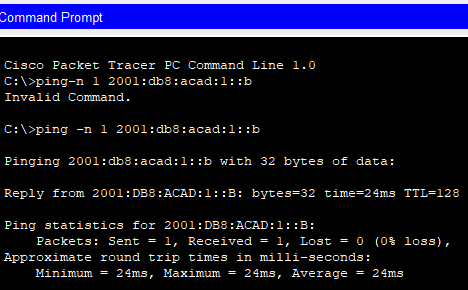
\includegraphics[width=0.8\textwidth]{11.png}
\end{figure}


\subsubsection*{(P1) En el panel de simulación utilizamos el botón forward hasta que aparezcan 13 mensajes en la ventana Event List como se observa en la figura 5. ¿Por qué están presentes los PDU NDP?}
\begin{figure}[h]
    \centering
    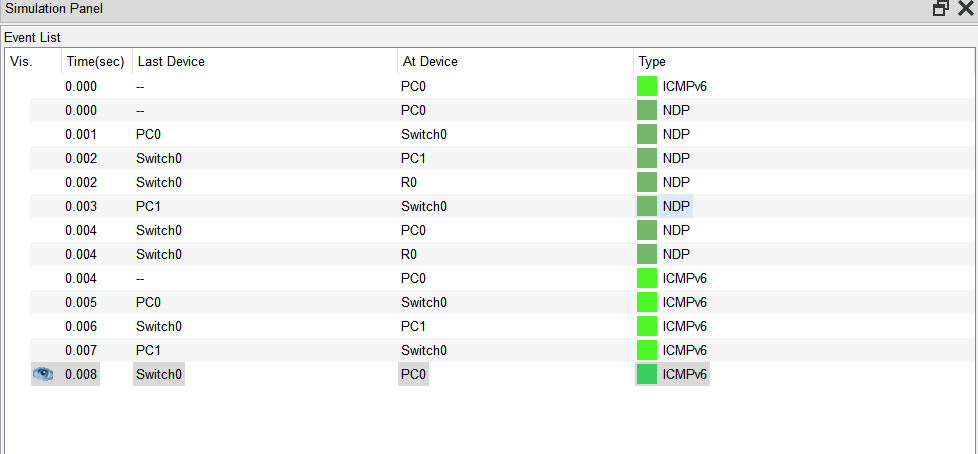
\includegraphics[width=0.8\textwidth]{12.png}
\end{figure}

Los mensajes del protocolo Neighbor Discovery Protocol (NDP) están presentes porque IPv6 no usa ARP como en IPv4. En su lugar, cuando PC0 intenta hacer ping a PC1, necesita conocer la dirección MAC correspondiente a la dirección IPv6 de destino (PC1). Como no la tiene en su caché de vecinos, genera un mensaje Neighbor Solicitation (NS) para obtenerla.

\subsubsection*{(P2) Seleccione el primer evento ICMPv6 en PC0. Observe la sección Out Layers del OSI Model ¿que tipo de mensaje es? Observe luego que direccionamiento aparece en L2. Una explicación sobre lo que ocurre a nivel L2 se obtiene con el botón Next Layer. Analize los campos relevantes y corrobore con la teoría.}
\begin{figure}[h]
    \centering
    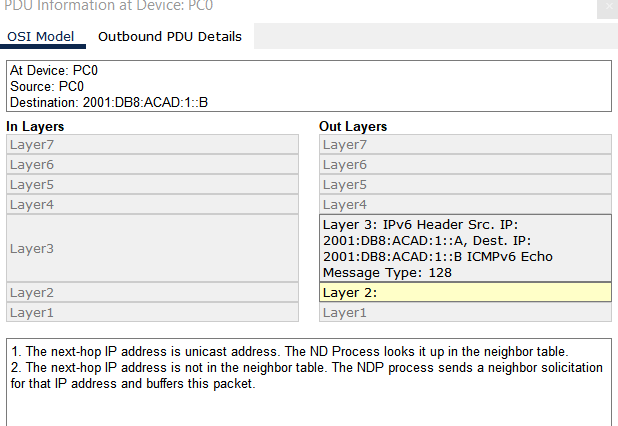
\includegraphics[width=0.8\textwidth]{13.png}
\end{figure}

\begin{itemize}
\item \textbf{Tipo de mensaje}: ICMPv6 Tipo 128 (Echo Request)
\item \textbf{Direccionamiento en Layer 2}:
La PC0 no conoce la MAC de la PC1, entonces inicia el proceso de Neighbor Discovery (NDP) enviando un Neighbor Solicitation (NS) a una dirección de multidifusión. Luego, PC1 responde con un Neighbor Advertisement (NA), proporcionando su MAC real.
\item \textbf{En layer 3}:
\begin{itemize}
\item Dirección origen: \dir{2001:DB8:ACAD:1::A} (Dirección de PC0)
\item Dirección destino: \dir{2001:DB8:ACAD:1::B} (Dirección de PC1)
\item Hop limit: 128

\end{itemize}
\end{itemize}
\begin{bytefield}{32}
    \bitheader{0-31} \\ % Encabezado de bits
    \bitbox{4}{VER 6} & \bitbox{8}{TRFC} & \bitbox{20}{FLOW LABEL} \\
    \bitbox{16}{PL: 108} & \bitbox{8}{NEXT: 0x3a} & \bitbox{8}{HOP LIMIT: 128} \\
    \bitbox{32}{SRC IP: 2001:DB8:ACAD:1::A} \\
    \wordbox{1}{ } \\
    \wordbox{1}{ } \\
    \bitbox{32}{DST IP: 2001:DB8:ACAD:1::B} \\
\end{bytefield}
\subsubsection*{(P3) Seleccione el proximo evento en PC0 del tipo NDP. ¿Qué ha cambiado en el direccionamiento L3 y L2? Cuando un host no conoce la dirección MAC del destino, IPv6 ND utiliza una dirección MAC especial de multidifusión 3333.XXXX.XXXX. Indague y profundice sobre cómo la utiliza.}
\begin{figure}[h]
    \centering
    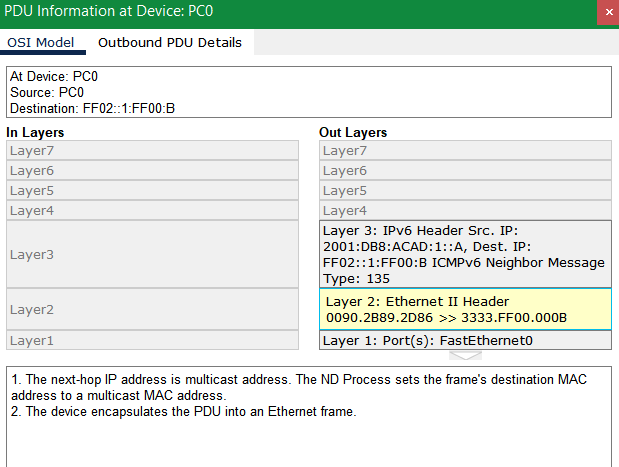
\includegraphics[width=0.8\textwidth]{15.png}
\end{figure}

\begin{itemize}
\item \textbf{En Capa 3 (L3 - IPv6)}: Ahora PC0 está enviando un mensaje de Neighbor Solicitation (NS) con la dirección de destino de PC1.
\item \textbf{En Capa 2 (L2 - Ethernet)}: Como PC0 no conoce la dirección MAC de PC1, envía el NS a una dirección MAC de multidifusión especial del tipo \dir{33:33:XX:XX:XX:XX}, donde los últimos 24 bits corresponden a los últimos 24 bits de la dirección IPv6 de PC1.
\end{itemize}

\paragraph*{¿Cómo se usa la dirección de multidifusión 3333.XXXX.XXXX?}
El prefijo \dir{33:33} es reservado para direcciones multidifusión en IPv6
.Los últimos 32 bits de la dirección MAC se derivan de la dirección IPv6 de destino,esto permite que sólo los dispositivos en la red local que tengan la dirección IPv6 en cuestión escuchen y respondan


\subsubsection*{(P4)  Seleccione el próximo evento en Switch0. ¿Hay diferencias entre las entradas y salidas en L2?}
\begin{figure}[h]
    \centering
    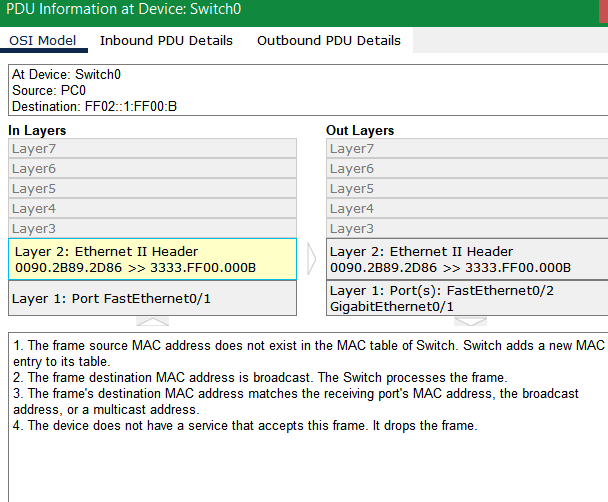
\includegraphics[width=0.8\textwidth]{16.png}
\end{figure}

Diferencias entre las entradas y salidas en L2:
El switch no cambia direcciones MAC de origen/destino,solo reenvía los paquetes a los puertos correctos en función de su tabla de direcciones MAC.Como la dirección MAC de destino es de multidifusión (\dir{33:33:XX:XX:XX:XX}), el switch reenvía el paquete a todas las interfaces activas, excepto la de donde provino.Una vez que PC1 responde con su MAC en un Neighbor Advertisement (NA), el switch puede actualizar su tabla MAC


\subsubsection*{(P5) Inspeccione los detalles salientes (Outbound PDU Details) en el primer evento en PC1 y anote los valores de las siguientes direcciones:
\begin{figure}[h]
    \centering
    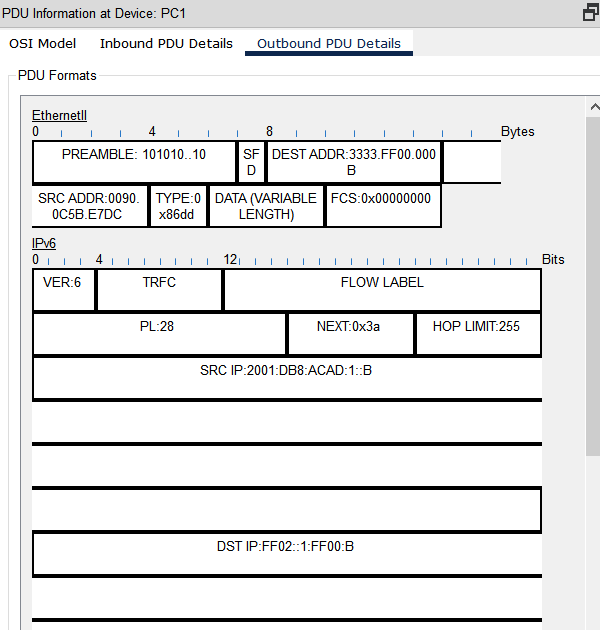
\includegraphics[width=0.8\textwidth]{17.png}
\end{figure}
}
\section*{EthernetII}
\begin{bytefield}{14} 
    \bitheader{0-13} \\
    \bitbox{8}{PREAMBLE: 101010..10} & \bitbox{8}{SF D} & \bitbox{16}{DEST ADDR: 3333.FF00.000} \\
    \bitbox{16}{SRC ADDR: 0090.0C5B E7DC} & \bitbox{16}{TYPE: 0x86dd} \\
    \bitbox{32}{DATA (VARIABLE LENGTH)} \\
    \bitbox{32}{FCS: 0x00000000} \\
\end{bytefield}
\section*{IPv6}
\begin{bytefield}{32}
    \bitheader{0-31} \\
    \bitbox{4}{VER: 6} & \bitbox{8}{TRFC} & \bitbox{20}{FLOW LABEL} \\
    \bitbox{16}{PL 28} & \bitbox{8}{NEXT: 0x3a} & \bitbox{8}{HOP LIMIT: 255} \\
    \bitbox{32}{SRC IP: 2001:DB8:ACAD:1::B} \\
    \bitbox{32}{} \\
    \bitbox{32}{} \\
    \bitbox{32}{DST IP: FF02::1:FF00:B} \\
\end{bytefield}

\begin{enumerate}
\item Ethernet Destination Address: \dir{3333.FF00.000B}
\item Ethernet Source Address: \dir{0090.0C5B.E7DC}
\item IPv6 Source Address: \dir{2001:DB8:ACAD:1::B}
\item IPv6 Destination Address: \dir{FF02::1:FF00:B}
\end{enumerate}

\subsubsection*{(P6) Seleccione el evento NDP en R0 y responda ¿por qué no hay información en Out Layers? Puede obtener más información leyendo los puntos 4 al 7 que aparecen al seleccionar varias veces Next Layer.}
\begin{figure}[h]
    \centering
    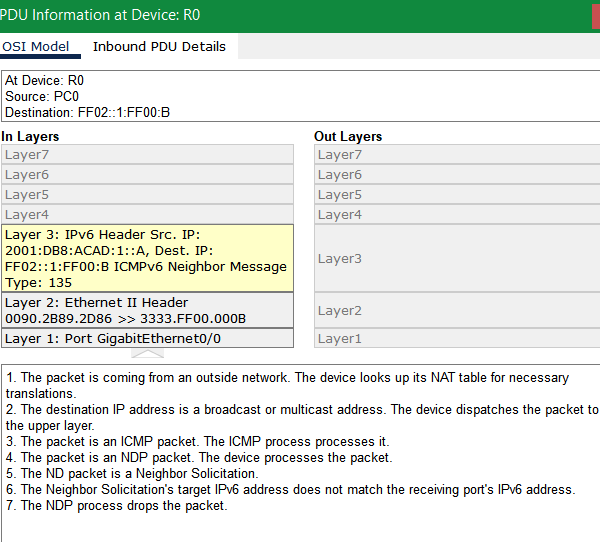
\includegraphics[width=0.8\textwidth]{18.png}
\end{figure}

Cuando un paquete se procesa pero no genera una respuesta, no va a haber una capa de salida. La razón principal es que el paquete fue descartado. Esto se debe a que el paquete no requiere una respuesta, ya que la dirección ya es conocida. Podemos darnos cuenta de esto en el punto 7: "The NDP process drops the packet"

\subsubsection*{(P7)  Seleccione el evento ICMPv6 próximo en PC0 ¿Podemos afirmar que ahora PC0 tiene toda la información para comunicarse con PC1?
}
\begin{figure}[h]
    \centering
    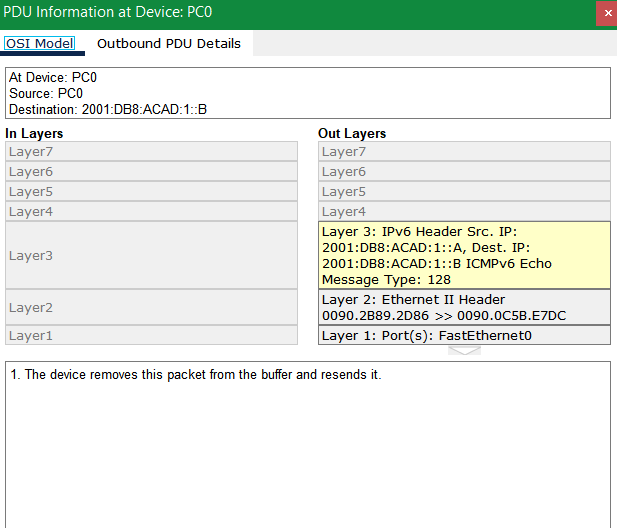
\includegraphics[width=0.8\textwidth]{19.png}
\end{figure}

Para que PC0 pueda comunicarse con PC1 correctamente en IPv6, necesita:
\begin{itemize}
\item Conocer la dirección IPv6 de PC1 (ya la tiene porque fue ingresada manualmente)
\item Saber la dirección MAC de PC1 (esto se obtiene a través de Neighbor Discovery Protocol - NDP)
\end{itemize}

Si en el evento de ICMPv6 en PC0 ya se está enviando un mensaje sin más consultas NDP previas, significa que PC0 ya aprendió la dirección MAC de PC1. En este caso, sí podemos afirmar que PC0 tiene toda la información necesaria para comunicarse con PC1.

\subsubsection*{(P8) Observe el próximo evento ICMPv6 de PC0. Este es el último evento que aparece en la lista. ¿Que tipo de mensaje ICMPv6 es?
\begin{figure}[h]
    \centering
    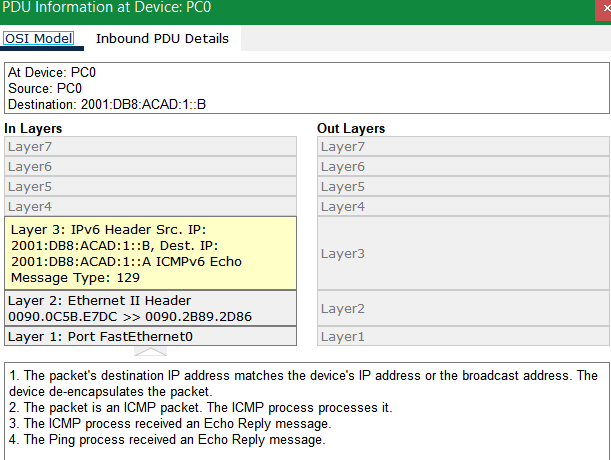
\includegraphics[width=0.8\textwidth]{20.png}
\end{figure}
}

Message Type 129: Echo Reply. Es un ping de vuelta, PC1 respondió con un mensaje tipo 129 (Echo Reply).

\subsubsection*{(P9)Ahora resetee la simulaci´on y desde la l´ ınea de comando de PC0 repita el ping a PC1. Utilice 5 veces el botón Forward para avanzar la simulaci´on y responde ¿Por qu´ e no hubo ning´ un evento NDP?}
\begin{figure}[h]
    \centering
    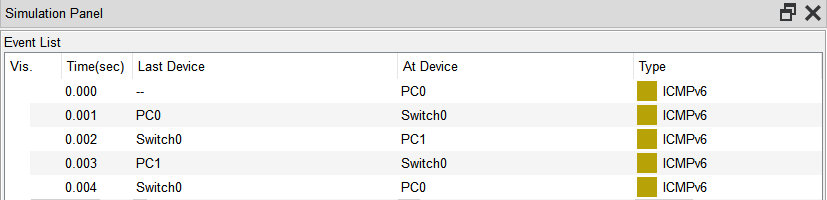
\includegraphics[width=0.8\textwidth]{21.png}
\end{figure}
Al hacer ping por segunda vez, el proceso NDP ya no es necesario porque las direcciones MAC ya fueron aprendidas y almacenadas en la caché de vecinos de PC0 y R0.

Cuando un host IPv6 necesita comunicarse con otro, primero revisa su caché de vecinos. Si la información aún está en la caché, simplemente reutiliza la dirección MAC y envía directamente el paquete ICMPv6 sin necesidad de resolver la MAC nuevamente con NDP.

\section*{2.2 Non Local Delivery}

\subsubsection*{(p1)Procedemos a borrar la informacion de vecindad en R0 y reseteamos la simulacion} Borramos la información de la vecindad del router R0 utilizando el comando:
\begin{lstlisting}
R0#clear Ipv6 neighbors
\end{lstlisting}

\subsubsection*{(p2) Realizamos un ping a la PC2 desde la consola de PC0} Realizamos un PING de la PC0 a la PC2 a través del comando:
\begin{lstlisting}
C:\>ping -n 1 2001:db8:acad:2::
\end{lstlisting}

\subsubsection*{(p3)} 
\begin{figure}[h]
    \centering
    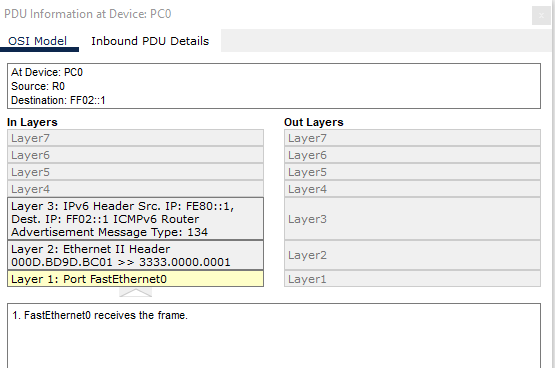
\includegraphics[width=0.8\textwidth]{23.png}
\end{figure}


\subsubsection*{(p4) Ahora analizamos el proximo evento NDP en PC0. ¿Que tipo de mensaje ND es y que direccion IPv6 de origen tiene? Ahora IPv6 NDP determinara la direccion destino para reenviar el ICMPv6. Los siguientes mensajes NDP cumplen una funcion similar a la analizada en la seccion anterior.} 
El evento NDP es un mensaje ND de tipo RA y tiene una dirección IPv6 de origen \dir{FE80::1}

\subsubsection*{(p5)Busque el proximo evento ICMPv6 en PC0 y verifique que posee toda la informacion para enviar el mensaje. ¿Cuales son las direcciones L2 en el que esta encapsulado? Explique.}
Direcciones L2 en el mensaje ICMPv6:

\begin{itemize}
    \item MAC de origen: \dir{0000.BD90.BC01}
    \item MAC de destino: \dir{3333.0000.0001}
\end{itemize}

\subsubsection*{(p7) Dirigase al proximo evento ICMPv6 en PC2. ¿cual es el tipo de mensaje ICMPv6 saliente y que informacion falta de L2? Elabore su respuesta}
El tipo de mensaje ICMPv6 saliente es un Echo Reply. En cuanto a la información faltante, falta la dirección MAC destino (de R0), por lo que PC2 debe realizar una solicitud de vecino para resolverla.

\subsubsection*{(p9)Resetee la simulacion y vuelva a enviar el ping. Utilice el boton Forward Capture 9 veces para completar el proceso de ping. ¿Hubo alg´ un evento NDP? Inspeccione el evento en PC2 ¿a que direccion MAC de destino se env´ ıa y porque?}
\begin{figure}[h]
    \centering
    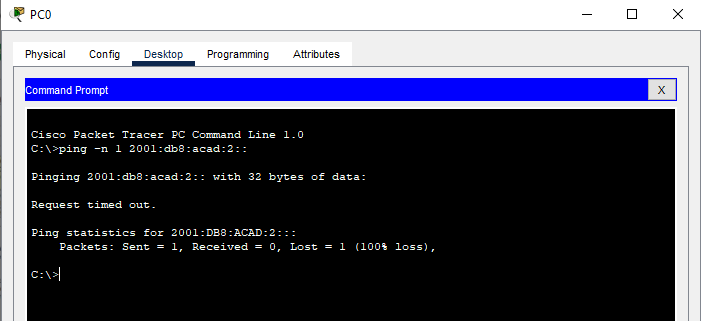
\includegraphics[width=0.8\textwidth]{22.png}
\end{figure}
El evento NPD tiene como dirección MAC de destino a R1 ya que es el default gateway para llegar a PC0

\subsubsection*{(p10) Regrese al modo realtime y examine los vecinos IPv6 de R0 y responda:
 1 ¿Cu´antas direcciones aparecen en la lista?
 2 ¿Con qu´ e dispositivos est´an asociadas estas direcciones?
 3 ¿Hay alguna entrada para PC1 en la lista? Justifique.}
Aparecen 3 direcciones en la lista. Estas están asociadas con Switch0, Switch1 y PC2. No hay entrada para PC1 en la tabla de vecinos de R0 porque no ha habido comunicación directa entre ellos

\subsubsection*{(p11) Realice un ping a PC1 desde R0 ¿que pasa al mirar nuevamente la lista?}
Al examinar nuevamente la lista de vecinos, ahora aparece una entrada para PC1, ya que el ping generó tráfico que permitió a R0 aprender la dirección MAC de PC1 mediante NDP.


\section*{3 Conclusiones}


\subsubsection*{1)¿Qué ventaja y desventajas plantea la autoconfiguración de IPv6?}
La autoconfiguracion de direcciones ipv6 mediante SLAAC simplifica la administracion de redes al eliminar la necesidad de configurar manualmente la dirección de cada dispositivo. Sin embargo,  esto podría ser desventajoso si en cambio se quiere dar un configuración más personalizada y específica en caso de que sea necesaria.

\subsubsection*{2)¿Qué tipos de mensajes se utilizan en la configuración vs el descubrimiento y cómo se relacionan?}

En la configuración se emiten mensajes del tipo Router Solicitation (\proto{RS}) y Router Advertisement (\proto{RA}) del protocolo ICMPv6. Mientras que por el otro lado, en el descubrimiento se emplean los mensajes de Neighbor Solicitation (\proto{NS}) y Neighbor Advertisement (\proto{NA}) dentro de Neighbor Discovery Protocol (\proto{NDP}).

La relación entre estas es evidente, la configuración permite a un host obtener su dirección IPv6 y la dirección del router, mientras que el descubrimiento de vecinos se usa para encontrar otros dispositivos en la misma red y resolver direcciones MAC, haciéndose posible la comunicación

\subsubsection*{3)¿Cuándo requiere un dispositivo el proceso de detección de vecinos IPv6?}

Cuando necesita comunicarse con otro dispositivo en la misma red local y no conoce su dirección MAC o si su caché de vecinos necesita ser actualizada.

\subsubsection*{4)¿Cómo ayuda un router a minimizar la cantidad de tráfico IPv6 Neighbor Discovery en una red?}

Almacenando información de vecinos en caché, evitando que los hosts tengan que enviar constantemente mensajes de descubrimiento de vecinos.

\subsubsection*{5)¿Cómo minimiza IPv6 el impacto del proceso ND en los hosts de red?}

Para minimizar el impacto del proceso Neighbor Solicitation en los hosts de red IPV6 almacena las direcciones MAC de los dispositivos vecinos para reducir las solicitudes de descubrimiento, realiza verificaciones rápidas y eficientes para evitar conflictos de direcciones y utiliza mensajes multicast en lugar de broadcast, reduciendo el tráfico innecesario.

\subsubsection*{6)¿En qué difiere el proceso de detección de vecinos cuando un host de destino está en la misma LAN y cuando está en una LAN remota?}

La diferencia entre el proceso de detección de vecinos cuando un host de destino está en la misma LAN y cuando está en una LAN remota es que cuando están en la misma LAN se usan mensajes Neighbor Solicitation y Neighbor Advertisement para resolver direcciones MAC locales. Mientras que en una LAN remota el tráfico pasa primero por un router. Si el destino está en otra red, se utilizan mensajes de enrutamiento y, potencialmente, protocolos de enrutamiento como OSPFv3 o EIGRP para IPv6.


\end{document}